\section{\textsc{Rohkostsalat mit Apfel}}

\subsection*{Zutaten für 2 Portionen:}

\begin{tabular}{p{7.5cm} p{7.5cm}}
	& \\
	\sfrac{1}{2} Weißkohlkopf & 3EL Olivenöl \\
	2 Karotten & 3EL Weißweinessig \\
	1 Äpfel & 1EL Salz \\
	\multicolumn{2}{l}{Pfeffer, Zucker, Kümmel nach Geschmack}
\end{tabular}

\subsection*{Serviervorschlag:}

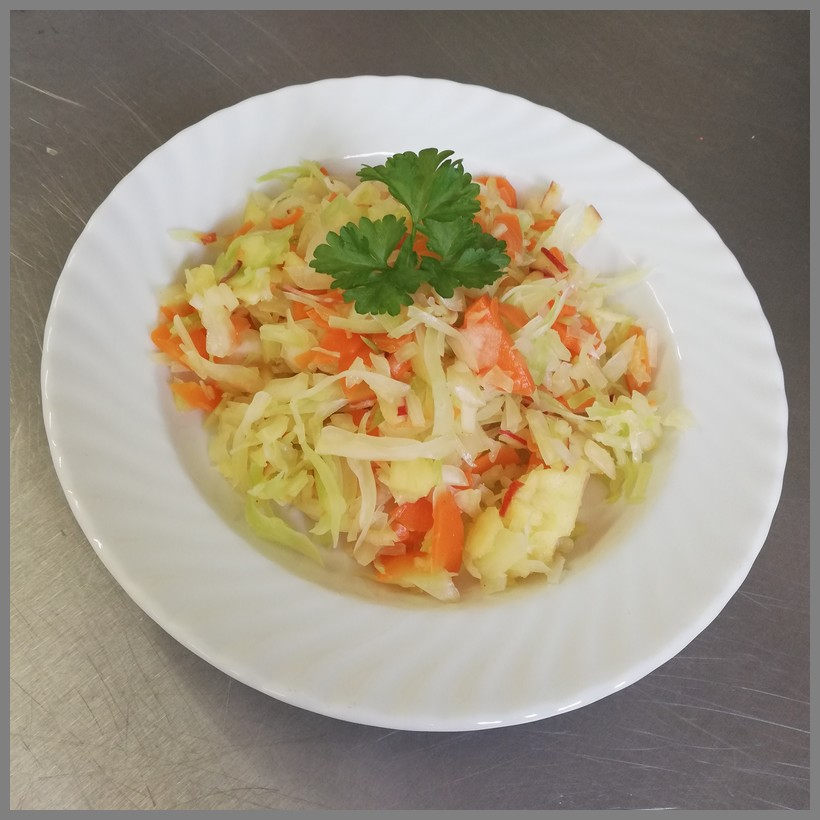
\includegraphics[width=\textwidth]{img/krautsalat_apfel.jpg} \cite{rohkostapfel}

\subsection*{So geht's:}
\begin{tabular}{p{15cm}}
	\\
	Den Weißkohl in dünne Streifen (Schnittform: Julienne) schneiden.\\
	Apfel und Karotten schälen und im Anschluss raspeln.\\
  Alles in eine große Schüssel geben.\\
	Salz, Essig \& Öl hinzufügen und solange fest kneten, bis der Kohl einen eigenen Saft bildet.\\
	Nun mit Pfeffer, Zucker und je nach Geschmack mit Kümmel würzen.\\
	Den Salat 1h ziehen lassen. Vor dem Servieren noch einmal abschmecken.
\end{tabular}
